% SpectralRelaxation 1.0
% Spectral Relaxation and Projective Mode Saturation
% J. Beau -- Cosmochrony Programme


\documentclass[12pt, a4paper]{article}

% --- packages ---
\usepackage[T1]{fontenc}
\usepackage[utf8]{inputenc}
\usepackage{amsmath, amssymb, amsthm}
\usepackage{hyperref}
\usepackage{geometry}
\usepackage{booktabs}
\usepackage{xcolor}
\usepackage{doi}
\usepackage{graphicx}

\geometry{margin=2.5cm}

% --- theorem environments ---
\theoremstyle{plain}
\newtheorem{proposition}{Proposition}[section]
\newtheorem{corollary}{Corollary}[section]
\newtheorem{lemma}{Lemma}[section]

\theoremstyle{definition}
\newtheorem{definition}{Definition}[section]
\newtheorem{hypothesis}{Hypothesis}[section]

\theoremstyle{remark}
\newtheorem{remark}{Remark}[section]

\title{Asymptotic Saturation of Projective Resolution:\\
Spectral Growth along the Projective Cascade}

\author{J\'er\^ome Beau\\[4pt]
\small Independent Researcher, Cosmochrony Project\\
\small \texttt{contact@cosmochrony.org}}

\date{\today}


\begin{document}

  \maketitle

  \begin{abstract}
    We investigate the spectral mechanism governing mode stabilisation in the
    Cosmochrony projective cascade framework.
    Starting from the admissibility condition defining the projective resolution
    $\Lambda_{\mathrm{proj}}$, we derive its dependence on the isoperimetric
    capacity of the cascade graph and show that
    $\Lambda_{\mathrm{proj}} \asymp h(G)^2$.
    For expander families satisfying spectral-isoperimetric saturation, this
    implies $\Lambda_{\mathrm{proj}} \asymp \lambda_2$.

    In the Lubotzky--Phillips--Sarnak (LPS) graph model with fixed prime $p$,
    the spectral gap converges to a constant, making $\Lambda_{\mathrm{proj}}$
    asymptotically static.
    In this regime, the stabilisation of modes is governed not by the admissibility
    threshold but by saturation of the cumulative spectral count below
    $\Lambda_{\mathrm{proj}}$.

    Combining this counting mechanism with the representation structure of ADE
    Cayley graphs yields a factorised prediction for mass ratios,
    \[
      \frac{\mathcal{M}_i}{\mathcal{M}_j}
      \;\propto\;
      \frac{F_{\mathrm{KM}}(\lambda_i)}{F_{\mathrm{KM}}(\lambda_j)}
      \cdot
      \frac{\dim\rho_{\lambda_j}}{\dim\rho_{\lambda_i}},
    \]
    where $F_{\mathrm{KM}}$ is the Kesten--McKay cumulative distribution function.
    Numerical evaluation shows that this single-level mechanism produces mass
    ratios of order unity and inverts the ordering expected from the admissibility
    envelope.
    We identify the asymptotic constancy of $\Lambda_{\mathrm{proj}}$ as the
    origin of both limitations, and establish that this structural obstacle
    historically motivated the O-series adoption of the Heisenberg BFS cascade.
    We further identify a two-regime growth law --- polynomial in the BFS shell
    regime, exponential in the trajectory-branching regime --- as a structural
    model of decelerated then accelerated expansion, compatible with recent DESI
    evidence for dynamical dark energy.
    The transfer of the exponential regime to the Heisenberg substrate is
    established at the level of projectively distinguishable histories in the
    trajectory-branching note~\cite{Beau2026tb}, which pins its canonical rate at
    $\log(1+\sqrt{2})$.

    \medskip
    \noindent\textbf{Keywords:}
    Spectral graph theory; Ramanujan graphs; Expander graphs; Cheeger inequality;
    Kesten--McKay distribution; Graph Laplacian spectrum; Emergent mass hierarchy;
    Projective cascade; Cosmological expansion
  \end{abstract}

  \clearpage
  \tableofcontents
  \newpage

  \clearpage
  \section{Introduction}
    \label{sec:intro}

    \subsection{The stratigraphic problem}
      \label{sec:intro:problem}

      The Cosmochrony framework~\cite{Cosmochrony} associates to each
      cascade rank $n$ an energy scale $E_n = E_{\mathrm{P}}/n$ and a spectral
      admissibility condition: a mode of eigenvalue $\lambda$ is projectable at rank
      $n$ if and only if $\lambda \leq \Lambda_{\mathrm{proj}}(n)$, where
      $\Lambda_{\mathrm{proj}}(n)$ is the projective resolution at that stage of the
      cascade.
      The \emph{stabilisation rank} of a mode is the first $n$ at which it ceases
      to be admissible, and the corresponding stabilisation energy is taken as a
      proxy for the physical mass of the associated particle sector.

      For this picture to produce a viable mass hierarchy, three conditions must hold
      simultaneously.
      First, the projective resolution must decrease with rank, so that earlier
      stabilisations correspond to higher masses.
      Second, the set of stabilisation ranks must be discrete, so that the spectrum
      of effective masses is not a continuum.
      Third, the inter-level separations must be large enough to account for the
      observed mass ratios between generations, which span five to seventeen orders
      of magnitude from the electron to the top quark.

      The first two conditions were addressed in~\cite{Beau2026a4}.
      The third -- which requires a quantitative law for $\Lambda_{\mathrm{proj}}(n)$
      -- was left as an open problem there and is the subject of the present paper.

    \subsection{What SpectralStratigraphy established}
      \label{sec:intro:stratigraphy}

      The companion paper~\cite{Beau2026a4} established two results that
      together constrain the form of $\Lambda_{\mathrm{proj}}(n)$ from above and
      below.

      \medskip
      \noindent\textbf{No-go for scalar calibration (Proposition~2
  of~\cite{Beau2026a4}).}
      A threshold of the form $E^*(\lambda) = E_0 \lambda^\beta$ cannot produce a
      discrete stratigraphic profile for any choice of parameters $(\alpha, \beta)$.
      This rules out any explanation of the discreteness of the generation spectrum
      by re-scaling or re-calibrating the energy-eigenvalue relation.
      The discretisation must therefore originate in the internal structure of the
      projective substrate.

      \medskip
      \noindent\textbf{Three-level structure from ADE binary groups
    (Proposition~3 of~\cite{Beau2026a4}).}
      For four specific pairs $(G, S)$ drawn from the binary tetrahedral, octahedral,
      and icosahedral groups -- $2T$ with order-3 generators, $2O$ with order-3
      generators, and $2I$ with order-4 or order-5 generators -- the Cayley graph
      Laplacian has exactly three distinct non-zero eigenvalues.
      Each eigenvalue level corresponds to a block of irreducible representations.
      Consequently, the stratigraphy defined by the Born--Infeld admissibility
      envelope $A^{\max}(\lambda) \propto 1/\sqrt{\lambda}$ produces exactly three
      stratigraphic classes, ordered by decreasing admissibility window.

      These two results together establish the following separation of roles, which
      is the central logical outcome of~\cite{Beau2026a4}:
      \begin{quote}
        \emph{Group topology determines the number of stratigraphic levels.
        Projective dynamics determines the inter-level separations.}
      \end{quote}

    \subsection{What remained open}
      \label{sec:intro:open}

      Despite the clean three-level structure, the numerical inter-level separations
      produced by the ADE examples are small: between $0.08$ and $0.18$ log-decades
      in cascade depth $\log n$, as reported in Table~2 of~\cite{Beau2026a4}.
      This is far too small to account for mass ratios of order $10^5$--$10^{17}$.

      The gap is not a defect of the group-theoretic mechanism.
      It reflects the fact that the spectral ratios $\lambda_\ell / \lambda_h$ for
      the ADE Cayley graphs lie in the range $[1.5, 2.0]$: the eigenvalue levels are
      spectrally close.
      Amplifying these small spectral differences into large mass ratios requires a
      rapidly growing function $\Lambda_{\mathrm{proj}}(n)$.

      The missing ingredient is therefore precisely the \emph{growth law} of
      $\Lambda_{\mathrm{proj}}(n)$ along the cascade trajectory.
      This law must be derived from within the framework, not imposed as an external
      ansatz: the no-go result rules out scalar power-law calibrations, and any
      other ad hoc choice would undermine the predictive content of the stratigraphy.

    \subsection{Aim and approach of the present paper}
      \label{sec:intro:aim}

      This paper proposes a derivation of $\Lambda_{\mathrm{proj}}(n)$ grounded in
      the global coherence properties of the cascade graph $G(n)$.
      The growth of $G(n)$ with~$n$ --- in the sense that $|V(G(n))| \sim n$ ---
      encodes the progressive unfolding of the observable algebra along the projective
      cascade: at each cascade rank the effective graph $G(n)$ represents the relational
      structure accessible to the projection~$\Pi$ at that depth, and its isoperimetric
      capacity controls which spectral modes of the substrate are projectively admissible.

      The key observation is that $\Lambda_{\mathrm{proj}}(n)$ is entirely controlled
      by the global projective flux bound $c_{\mathrm{BI}}(n)$:
      \[
        \Lambda_{\mathrm{proj}}(n) = \frac{c_{\mathrm{BI}}(n)^2}{A_{\min}^2}.
      \]
      The dynamical question reduces to: \emph{how does $c_{\mathrm{BI}}(n)$ depend on the
  cascade rank?}
      We argue that $c_{\mathrm{BI}}(n)$ is bounded by the isoperimetric capacity of $G(n)$,
      measured by the Cheeger constant $h(G(n))$, which is in turn controlled by the
      algebraic connectivity $\lambda_2(n)$ via the discrete Cheeger inequality.

      The logical chain of the derivation is:
      \[
        \text{global coherence}
        \;\longrightarrow\; c_{\mathrm{BI}}(n)
        \;\longrightarrow\; h\bigl(G(n)\bigr)
        \;\longrightarrow\; \lambda_2(n)
        \;\longrightarrow\; \Lambda_{\mathrm{proj}}(n).
      \]
      Two structural hypotheses are required: a \emph{projective coherence closure}
      (Hypothesis~\ref{hyp:closure}) and a \emph{spectral-isoperimetric saturation}
      condition (Hypothesis~\ref{hyp:saturation}).
      Both are stated explicitly and treated as independent structural postulates.

      The main results of the paper are as follows.
      \begin{itemize}
        \item \textbf{Proposition~\ref{prop:Lambda-h}}:
        $\Lambda_{\mathrm{proj}}(n) \asymp h(G(n))^2$ under Hypothesis~\ref{hyp:closure}
        alone.
        \item \textbf{Corollary~\ref{cor:cheeger-enclosure}}:
        $\lambda_2(n)^2 \lesssim \Lambda_{\mathrm{proj}}(n) \lesssim \lambda_2(n)$
        via the Cheeger inequality, with no additional hypotheses.
        \item \textbf{Corollary~\ref{cor:linear-law}}:
        $\Lambda_{\mathrm{proj}}(n) \asymp \lambda_2(n)$ under both hypotheses.
      \end{itemize}
      The programmatic consequence is that the problem of inter-generation mass ratios
      reduces to the problem of computing $\lambda_2(n)$ along the cascade trajectory.

    \subsection{Structure of the paper}
      \label{sec:intro:structure}

      Section~\ref{sec:framework} establishes the formal framework.
      Section~\ref{sec:model} introduces the LPS graph model and identifies the
      cascade index.
      Section~\ref{sec:spectral} analyses the spectral behaviour of LPS graphs and
      derives the growth law for $N(\lambda; n)$.
      Section~\ref{sec:amplification} evaluates the predicted mass ratios numerically.
      Section~\ref{sec:discussion} discusses limitations and open directions.
      Section~\ref{sec:conclusion} concludes.

    \subsection{Position within the Cosmochrony programme}
      \label{sec:intro:position}

      This paper occupies a specific historical and logical position within the
      Cosmochrony programme.

      \medskip
      \noindent\textbf{Historical role.}
      The structural negative result established here --- that
      $\Lambda_{\mathrm{proj}}$ is asymptotically static in the LPS model at fixed
      prime~$p$ --- identified the obstacle that motivated the O-series to adopt a
      different cascade model.
      Rather than a family of growing graphs $\{G(n)\}_{n \geq 1}$, the O-series
      works within a single fixed Heisenberg Cayley graph
      $\mathrm{Heis}_3(\mathbb{Z}/q\mathbb{Z})$, explored via BFS shells.
      In that setting, the analogue of $\Lambda_{\mathrm{proj}}(n)$ is the pair
      capacity $\sigma_{\mathrm{pair}}(n)$, which decays along the BFS cascade rather
      than saturating.
      The structural obstacle identified here --- the need for a dynamical threshold
      --- is precisely what the Heisenberg BFS model resolves.

      \medskip
      \noindent\textbf{Connection to relational admissibility.}
      The Foundation companion paper~\cite{Beau2026m} establishes that
      admissibility is never an absolute predicate of an observable state $O_n$, but
      a relational constraint on transitions: $O_n \in \mathcal{A}(O_{n-1})$, where
      $\mathcal{A}(O_{n-1})$ is the admissible neighbourhood from the preceding state.
      In the spectral language of this paper, $\Lambda_{\mathrm{proj}}(n)$ is the
      spectral expression of $\mathcal{A}(O_{n-1})$: it encodes which modes are
      reachable from the current projective position.
      The asymptotic constancy of $\Lambda_{\mathrm{proj}}$ in the LPS model reflects
      the fact that the LPS cascade graph does not vary its admissible neighbourhood
      as a function of the reached state.
      A dynamical $\Lambda_{\mathrm{proj}}(n)$ corresponds, in Foundation language, to
      a cascade in which $\mathcal{A}(O_n) \neq \mathcal{A}(O_{n-1})$ generically ---
      which is guaranteed by the non-trivial BFS shell structure of
      $\mathrm{Heis}_3(\mathbb{Z}/q\mathbb{Z})$.

      \medskip
      \noindent\textbf{Logical contribution.}
      The present paper contributes three elements to the broader programme:
      the isoperimetric law $\Lambda_{\mathrm{proj}} \asymp h(G)^2$
      (Proposition~\ref{prop:Lambda-h}), the spectral analysis of LPS graphs via the
      Kesten--McKay distribution, and the identification of direction~(O1) ---
      allowing $p(n) \to \infty$ jointly with~$n$ --- as the natural candidate for a
      dynamical cosmological threshold compatible with the observed mass ordering.
      The development of that cosmological model is carried forward by the O-series.
  \section{Formal Framework}
    \label{sec:framework}

    \subsection{Notation and basic objects}
      \label{sec:framework:notation}

      Throughout this paper, $n \in \mathbb{N}_{>0}$ denotes the \emph{cascade rank},
      an integer-valued depth parameter indexing successive stages of the projective cascade.
      It is distinct from the cardinality of any group or graph.
      The energy available at rank $n$ is
      \begin{equation}
        \label{eq:energy-rank}
        E_n \;=\; \frac{E_{\mathrm{P}}}{n},
      \end{equation}
      where $E_{\mathrm{P}}$ is the Planck energy, in agreement with the cascade
      scaling of~\cite{Beau2026a4}.

      Let $G(n)$ denote the \emph{effective cascade graph} at rank $n$: a
      connected, $d(n)$-regular, undirected graph encoding the relational structure
      at stage~$n$.
      The vertex set is $V(n)$, the edge set $E(n)$, and the normalised graph
      Laplacian is $L_{G(n)}$, with eigenvalues
      $0 = \mu_0 < \mu_1 \leq \mu_2 \leq \cdots$.
      The \emph{algebraic connectivity} (Fiedler value) of $G(n)$ is
      \begin{equation}
        \label{eq:fiedler}
        \lambda_2(n) \;:=\; \mu_1\bigl(L_{G(n)}\bigr) \;>\; 0.
      \end{equation}
      The \emph{Cheeger constant} of $G(n)$ is
      \begin{equation}
        \label{eq:cheeger-def}
        h\bigl(G(n)\bigr)
        \;:=\;
        \min_{\substack{S \subset V(n) \\ 0 < |S| \leq |V(n)|/2}}
        \frac{|\partial S|}{|S|},
      \end{equation}
      where $\partial S$ is the set of edges with exactly one endpoint in $S$.

    \subsection{Projective admissibility and flux bound}
      \label{sec:framework:admissibility}

      Following~\cite{Beau2026a1, Beau2026a4}, a spectral mode
      of eigenvalue $\lambda$ is \emph{projectively admissible} at rank $n$ if the
      maximal effective amplitude supported by the projective flux bound
      $c_{\mathrm{BI}}(n) > 0$ satisfies
      \begin{equation}
        \label{eq:admissibility-envelope}
        A^{\max}(\lambda, n)
        \;:=\; \frac{c_{\mathrm{BI}}(n)}{\sqrt{\lambda}}
        \;\geq\; A_{\min},
      \end{equation}
      where $A_{\min} > 0$ is a fixed scale independent of $n$.
      The \emph{projective resolution} at rank $n$ is
      \begin{equation}
        \label{eq:Lambdaproj-def}
        \Lambda_{\mathrm{proj}}(n)
        \;:=\;
        \sup\bigl\{\lambda > 0 : A^{\max}(\lambda,n) \geq A_{\min}\bigr\}
        \;=\; \frac{c_{\mathrm{BI}}(n)^2}{A_{\min}^2}.
      \end{equation}
      All dependence of $\Lambda_{\mathrm{proj}}(n)$ on the cascade rank is
      carried entirely by $c_{\mathrm{BI}}(n)$.

    \subsection{Structural hypotheses}
      \label{sec:framework:hypotheses}

      \begin{hypothesis}[Projective coherence closure]
        \label{hyp:closure}
        The global projective flux bound satisfies
        \begin{equation}
          \label{eq:cchi-h}
          c_{\mathrm{BI}}(n) \;\asymp\; h\bigl(G(n)\bigr),
        \end{equation}
        with positive constants independent of~$n$.
      \end{hypothesis}

      \noindent
      Hypothesis~\ref{hyp:closure} is a closure assumption: it identifies the
      projective flux capacity with the isoperimetric capacity of the cascade graph.
      It is not derived from the internal dynamics of $G(n)$ and must be treated as
      an independent structural postulate.

      \begin{hypothesis}[Spectral-isoperimetric saturation]
        \label{hyp:saturation}
        Along the cascade trajectory,
        \begin{equation}
          \label{eq:saturation}
          h\bigl(G(n)\bigr)^2 \;\asymp\; \lambda_2(n),
        \end{equation}
        with constants independent of~$n$.
      \end{hypothesis}

      \noindent
      Hypothesis~\ref{hyp:saturation} holds when $G(n)$ belongs to a quasi-expander
      family in which $h \asymp \sqrt{\lambda_2}$ up to bounded factors.
      It is logically independent of Hypothesis~\ref{hyp:closure}.

    \subsection{Main results}
      \label{sec:framework:results}

      \begin{proposition}[Projective resolution from isoperimetric capacity]
        \label{prop:Lambda-h}
        Under Hypothesis~\ref{hyp:closure},
        \begin{equation}
          \label{eq:Lambda-h2}
          \Lambda_{\mathrm{proj}}(n) \;\asymp\; h\bigl(G(n)\bigr)^2.
        \end{equation}
      \end{proposition}

      \begin{proof}
        Immediate from~\eqref{eq:Lambdaproj-def} and~\eqref{eq:cchi-h}:
        $\Lambda_{\mathrm{proj}}(n) = c_{\mathrm{BI}}(n)^2/A_{\min}^2
        \asymp h(G(n))^2/A_{\min}^2$.
      \end{proof}

      \begin{corollary}[Cheeger enclosure for the projective resolution]
        \label{cor:cheeger-enclosure}
        For a $d(n)$-regular graph, the discrete Cheeger inequality~\cite{Chung1997}
        \begin{equation}
          \label{eq:cheeger-ineq}
          \frac{\lambda_2(n)}{2} \;\leq\; h\bigl(G(n)\bigr) \;\leq\; \sqrt{2\,\lambda_2(n)}
        \end{equation}
        combined with Proposition~\ref{prop:Lambda-h} gives
        \begin{equation}
          \label{eq:Lambda-enclosure}
          \frac{\lambda_2(n)^2}{4\,A_{\min}^2}
          \;\lesssim\; \Lambda_{\mathrm{proj}}(n)
          \;\lesssim\; \frac{2\,\lambda_2(n)}{A_{\min}^2}.
        \end{equation}
      \end{corollary}

      \begin{remark}
        The enclosure~\eqref{eq:Lambda-enclosure} is the sharpest consequence of
        Cheeger's inequality alone.
        The lower bound is quadratic and the upper bound is linear in $\lambda_2(n)$;
        no further tightening is possible without additional hypotheses on $G(n)$.
      \end{remark}

      \begin{corollary}[Linear projective-resolution law]
        \label{cor:linear-law}
        Under Hypotheses~\ref{hyp:closure} and~\ref{hyp:saturation},
        \begin{equation}
          \label{eq:Lambda-linear}
          \Lambda_{\mathrm{proj}}(n) \;\asymp\; \lambda_2(n).
        \end{equation}
      \end{corollary}

      \begin{proof}
        Combine Proposition~\ref{prop:Lambda-h} with Hypothesis~\ref{hyp:saturation}.
      \end{proof}

      \noindent
      Its physical content is that the maximal projectable eigenvalue at rank $n$ is
      controlled, up to bounded factors, by the algebraic connectivity of the
      effective cascade graph.

    \subsection{Dynamic extension: spectral counting and stabilisation}
      \label{sec:framework:dynamic}

      \begin{definition}[Spectral counting function]
        \label{def:counting}
        \begin{equation}
          \label{eq:counting-def}
          N(\lambda; n)
          \;:=\; \bigl|\bigl\{k : \lambda_k\bigl(G(n)\bigr) \leq \lambda\bigr\}\bigr|,
        \end{equation}
        where eigenvalues are counted with multiplicity.
      \end{definition}

      \begin{definition}[Projectable mode count]
        \label{def:Nproj}
        \begin{equation}
          \label{eq:Nproj-def}
          N_{\mathrm{proj}}(n)
          \;:=\; N\bigl(\Lambda_{\mathrm{proj}};\, n\bigr).
        \end{equation}
      \end{definition}

      \noindent
      $\Lambda_{\mathrm{proj}}$ fixes the spectral support of projectable modes;
      $N_{\mathrm{proj}}(n)$ counts how many such modes exist at rank $n$.
      These are independent quantities: $\Lambda_{\mathrm{proj}}$ depends on
      $c_{\mathrm{BI}}(n)$, while $N_{\mathrm{proj}}(n)$ depends on the spectral density of
      $G(n)$.

      \begin{hypothesis}[Representational saturation]
        \label{hyp:saturation-rep}
        A spectral mode at eigenvalue level $\lambda_i$ of the ADE substrate graph
        stabilises when its cumulative spectral count reaches the dimension of the
        corresponding irreducible representation block:
        \begin{equation}
          \label{eq:saturation-condition}
          M(\lambda_i) \;:=\; k\,\dim \rho_{\lambda_i},
        \end{equation}
        where $k \in \mathbb{N}_{>0}$ is a universal constant independent of $i$.
      \end{hypothesis}

      \begin{definition}[Stabilisation rank]
        \label{def:nproj}
        Under Hypothesis~\ref{hyp:saturation-rep},
        \begin{equation}
          \label{eq:nproj-def}
          n_{\mathrm{proj}}(\lambda_i)
          \;:=\; \inf\bigl\{n \in \mathbb{N}_{>0} :
          \lambda_i \leq \Lambda_{\mathrm{proj}}
          \;\text{ and }\;
          N(\lambda_i;\, n) \geq k\,\dim\rho_{\lambda_i}
          \bigr\}.
        \end{equation}
        The effective stabilisation mass is
        \begin{equation}
          \label{eq:mass-def}
          \mathcal{M}_i \;\propto\; \frac{E_{\mathrm{P}}}{n_{\mathrm{proj}}(\lambda_i)}.
        \end{equation}
      \end{definition}

      \begin{remark}[Separation of roles]
  The condition $\lambda_i \leq \Lambda_{\mathrm{proj}}$ is a support condition
  governing which modes can stabilise; $N(\lambda_i; n) \geq k\,\dim\rho_{\lambda_i}$
  is a saturation condition governing at which rank.
  When $\Lambda_{\mathrm{proj}}$ is asymptotically constant, the support
  condition reduces to a fixed constraint and all dynamics arises from the
  saturation condition.
      \end{remark}
  \section{Choice of a Cascade-Graph Model}
    \label{sec:model}

    \subsection{Requirements on the cascade graphs}
      \label{sec:model:requirements}

      The following properties are necessary for a family $\{G(n)\}_{n \geq 1}$ to
      be consistent with the projective cascade picture.

      \medskip
      \noindent\textbf{(R1) Vertex-transitivity.}
      The projection must not privilege any node; $G(n)$ must be vertex-transitive
      or quasi-homogeneous, so that $\lambda_2(n)$ is a well-defined global quantity.

      \medskip
      \noindent\textbf{(R2) Bounded degree.}
      The local relational flux capacity is finite, so $d(n)$ must remain bounded
      (or grow at most logarithmically) along the cascade.

      \medskip
      \noindent\textbf{(R3) Non-vanishing algebraic connectivity.}
      $\lambda_2(n) > 0$ must hold for all $n$, ensuring a coherent global
      projection.

      \medskip
      \noindent\textbf{(R4) Controlled spectral gap.}
      $\lambda_2(n)$ must admit explicit analytic lower bounds.

      \medskip
      \noindent\textbf{(R5) Constructibility as an explicit sequence.}
      The family must admit an explicit indexing compatible with the cascade rank $n$.

    \subsection{Candidate families and selection of LPS graphs}
      \label{sec:model:candidates}

      Random regular graphs satisfy (R1)--(R4) only in probability and not
      constructively, failing (R5).
      Cayley graphs of finite groups satisfy (R1) and (R4) for families with
      controlled character sums, but generic sequences need not satisfy (R3).
      Explicit expander families satisfy all five requirements by construction.
      Among expanders, \emph{near-Ramanujan} families are optimal: the Alon--Boppana
      theorem~\cite{Alon1986} bounds $\lambda_2 \leq 1 - 2\sqrt{d-1}/d + o(1)$, and
      Ramanujan graphs achieve this bound exactly.

      The Lubotzky--Phillips--Sarnak (LPS) construction~\cite{LPS1988} provides the
      only currently known explicit infinite families of Ramanujan graphs, and is
      the natural canonical choice satisfying all five requirements.

    \subsection{LPS graphs}
      \label{sec:model:lps}

      Let $p$ and $q$ be distinct odd primes, both congruent to $1 \pmod{4}$.
      The LPS graph $X^{p,q}$ is a $(p+1)$-regular Cayley graph on
      $\mathrm{PSL}(2, \mathbb{F}_q)$, with
      \begin{equation}
        \label{eq:lps-order}
        \bigl|V(X^{p,q})\bigr|
        \;=\; \tfrac{1}{2}\,q(q^2 - 1).
      \end{equation}
      The Ramanujan property gives, for the normalised Laplacian,
      \begin{equation}
        \label{eq:ramanujan-laplacian}
        \lambda_2\bigl(X^{p,q}\bigr)
        \;\geq\; 1 - \frac{2\sqrt{p}}{p+1},
      \end{equation}
      uniformly in $q$.
      All five requirements (R1)--(R5) are satisfied.

      \begin{remark}[Laplacian normalisation]
  Throughout this paper, $L_G = I - A/d$ denotes the normalised graph
  Laplacian, with eigenvalues in $[0,2]$.
  The Cheeger inequality~\eqref{eq:cheeger-ineq} and the Ramanujan
  bound~\eqref{eq:ramanujan-laplacian} use this convention consistently.
      \end{remark}

    \subsection{Identification of the cascade index}
      \label{sec:model:index}

      The physical identification is
      \begin{equation}
        \label{eq:index-id}
        n \;\sim\; \bigl|V\bigl(G(n)\bigr)\bigr|,
      \end{equation}
      interpreting the cascade depth as proportional to the number of active
      relational nodes.
      For the LPS family at fixed $p$,
      \begin{equation}
        \label{eq:index-lps}
        n \;\sim\; \tfrac{1}{2}\,q(q^2 - 1) \;\sim\; q^3/2
        \qquad (q \to \infty),
      \end{equation}
      so $q \sim (2n)^{1/3}$.
      Alternative identifications ($n \sim |E(G(n))|$, $n \sim \log|V|$) are
      discussed in Section~\ref{sec:discussion}.
  \section{Spectral Behaviour of LPS Graphs}
    \label{sec:spectral}

    \subsection{Algebraic connectivity along the cascade trajectory}
      \label{sec:spectral:lambda2}

      Fix $p$ and let $q \to \infty$.
      From~\eqref{eq:ramanujan-laplacian} and the Alon--Boppana
      bound~\cite{Alon1986},
      \begin{equation}
        \label{eq:lambda2-limit}
        \lambda_2(n) \;\longrightarrow\; \lambda_2^*(p)
        \;:=\; 1 - \frac{2\sqrt{p}}{p+1} \;>\; 0.
      \end{equation}

      \begin{proposition}[Asymptotic constancy of $\Lambda_{\mathrm{proj}}$]
        \label{prop:Lambda-constant}
        Under Hypotheses~\ref{hyp:closure} and~\ref{hyp:saturation}, for the LPS
        family at fixed $p$,
        \begin{equation}
          \label{eq:Lambda-constant}
          \Lambda_{\mathrm{proj}}(n) \;\longrightarrow\; \Lambda_0(p)
          \;:=\; \frac{C\,\lambda_2^*(p)}{A_{\min}^2}
          \qquad \text{as } n \to \infty.
        \end{equation}
      \end{proposition}

      \noindent
      Proposition~\ref{prop:Lambda-constant} shows that the admissibility threshold
      is asymptotically static in this model.
      The dynamical variable driving stabilisation is therefore the saturation
      condition $N(\lambda_i; n) \geq k\,\dim\rho_{\lambda_i}$, not the variation
      of $\Lambda_{\mathrm{proj}}$.

    \subsection{Kesten--McKay spectral density}
      \label{sec:spectral:kesten}

      As $q \to \infty$ with $p$ fixed, the empirical spectral measure of
      $L_{X^{p,q}}$ converges weakly to the \emph{Kesten--McKay
  measure}~\cite{McKay1981,Kesten1959}
      \begin{equation}
        \label{eq:kesten-mckay}
        \mathrm{d}\mu_{\mathrm{KM}}^{(p)}(\lambda)
        \;=\; \rho_{\mathrm{KM}}^{(p)}(\lambda)\,\mathrm{d}\lambda,
        \qquad
        \rho_{\mathrm{KM}}^{(p)}(\lambda)
        \;=\; \frac{(p+1)\sqrt{4p - (p+1)^2(1-\lambda)^2}}
        {2\pi\,p\,\bigl(1 - (1-\lambda)^2\bigr)},
      \end{equation}
      supported on $[\lambda_-, \lambda_+]$ with
      $\lambda_\pm = 1 \mp 2\sqrt{p}/(p+1)$.
      The density is symmetric about $\lambda = 1$:
      $\rho_{\mathrm{KM}}(\lambda) = \rho_{\mathrm{KM}}(2 - \lambda)$.

      \begin{figure}[h]
        \centering
        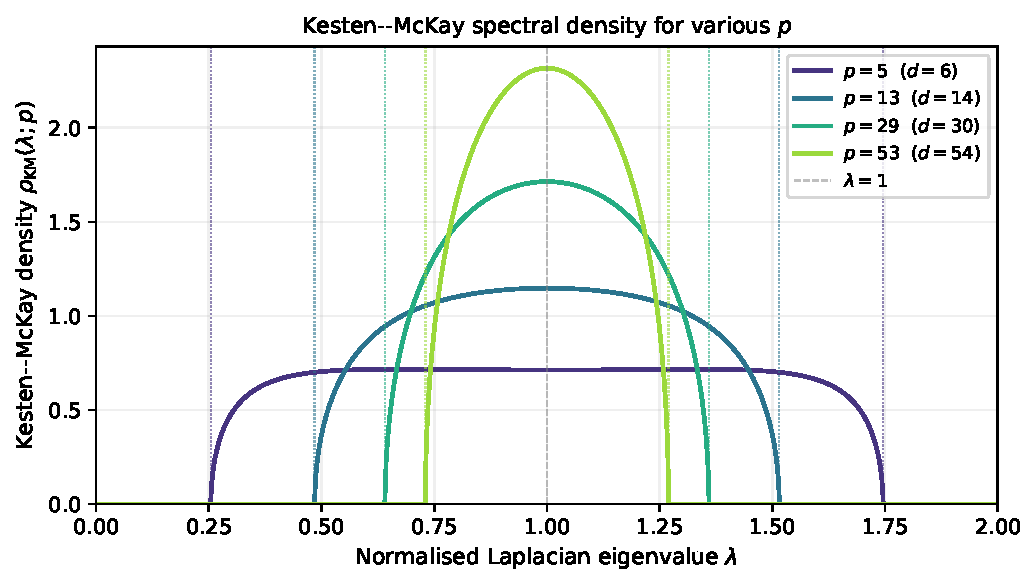
\includegraphics[width=0.82\textwidth]{../code/fig1_km_density}
        \caption{Kesten--McKay spectral density $\rho_{\mathrm{KM}}^{(p)}(\lambda)$
          for $(p+1)$-regular graphs with $p \in \{5, 13, 29, 53\}$.
          The support $[\lambda_-, \lambda_+]$ narrows as $p$ grows.
          Dashed vertical lines mark the three normalised eigenvalue levels of
          the $2I$ ord-5 ADE case ($\lambda_1 = 20/24$, $\lambda_2 = 1$,
          $\lambda_3 = 30/24$).
          All three levels lie inside the support for $p \leq 53$; the structural
          identity $F_{\mathrm{KM}}(1) = 1/2$ follows from the symmetry of the
          density about $\lambda = 1$.}
        \label{fig:km-density}
      \end{figure}

      \begin{remark}[Relation to the $S^3$ spectral measure]
  As $p \to \infty$, the Kesten--McKay measure converges to the spectral
  measure of the $S^3$ Laplacian~\cite{Beau2026a1}.
  The LPS family therefore interpolates between the discrete Ramanujan regime
  and the $S^3$ continuum.
      \end{remark}

    \subsection{Monotonicity and linear growth of the spectral counting function}
      \label{sec:spectral:counting}

      Write $F_{\mathrm{KM}}(\lambda) := \mu_{\mathrm{KM}}^{(p)}((-\infty, \lambda])$
      for the cumulative distribution function.
      By weak convergence and the identification~\eqref{eq:index-id}:
      \begin{equation}
        \label{eq:counting-linear}
        N(\lambda;\, n) \;\sim\; F_{\mathrm{KM}}(\lambda)\cdot n
        \qquad (n \to \infty).
      \end{equation}

      \begin{lemma}[Monotonicity]
        \label{lem:monotonicity}
        For $\lambda$ in the interior of $[\lambda_-, \lambda_+]$, $N(\lambda; n)$
        is strictly increasing in $n$ for all sufficiently large $n$.
      \end{lemma}

      \begin{proof}
        Since $F_{\mathrm{KM}}(\lambda) > 0$ for $\lambda$ in the interior of the
        support and $|V(G(n))| \sim n$ is strictly increasing,
        $N(\lambda;n) \sim F_{\mathrm{KM}}(\lambda)\cdot n$ is strictly increasing.
      \end{proof}

      \begin{proposition}[Linear growth of projectable mode count]
        \label{prop:Nproj-linear}
        For the LPS family at fixed $p$ and $\lambda \leq \Lambda_0(p)$,
        \begin{equation}
          \label{eq:Nproj-linear}
          N(\lambda;\, n) \;\sim\; F_{\mathrm{KM}}(\lambda)\cdot n
          \qquad \text{as } n \to \infty.
        \end{equation}
      \end{proposition}

      \noindent
      For the three ADE eigenvalue levels $\lambda_1 < \lambda_2 < \lambda_3$
      of~\cite{Beau2026a4}, define
      \begin{equation}
        \label{eq:KM-coefficients}
        c_i(p) \;:=\; F_{\mathrm{KM}}(\lambda_i)
        \;=\; \int_{\lambda_-}^{\lambda_i} \rho_{\mathrm{KM}}^{(p)}(x)\,\mathrm{d}x,
        \qquad i = 1,2,3,
      \end{equation}
      satisfying $0 < c_1(p) < c_2(p) < c_3(p) \leq 1$.
      Since $\lambda_2^{\mathrm{norm}} = 1$ for all three-level ADE cases and
      $F_{\mathrm{KM}}(1) = 1/2$ by symmetry of the Kesten--McKay density,
      \begin{equation}
        \label{eq:c2-universal}
        c_2(p) \;=\; \tfrac{1}{2}
        \qquad \text{for all } p.
      \end{equation}
      This is a structural identity, not a numerical coincidence.

    \subsection{Stabilisation ranks and mass formula}
      \label{sec:spectral:stabilisation}

      By Lemma~\ref{lem:monotonicity}, Definition~\ref{def:nproj} is well-posed.
      Inverting Proposition~\ref{prop:Nproj-linear}:
      \begin{equation}
        \label{eq:nproj-value}
        n_{\mathrm{proj}}(\lambda_i)
        \;\sim\; \frac{k\,\dim\rho_{\lambda_i}}{c_i(p)}.
      \end{equation}
      The effective stabilisation mass and inter-generation mass ratio are therefore
      \begin{equation}
        \label{eq:mass-formula}
        \mathcal{M}_i
        \;\sim\; \frac{c_i(p)\,E_{\mathrm{P}}}{k\,\dim\rho_{\lambda_i}},
        \qquad
        \frac{\mathcal{M}_i}{\mathcal{M}_j}
        \;=\; \frac{c_i(p)}{c_j(p)}\cdot
        \frac{\dim\rho_{\lambda_j}}{\dim\rho_{\lambda_i}}.
      \end{equation}
      The universal constant $k$ cancels in all ratios.
      The first factor $c_i/c_j$ is determined by the spectral geometry of the LPS
      substrate; the second factor $\dim\rho_j/\dim\rho_i$ is determined by the
      representation theory of the ADE group.
      The two mechanisms are independent and act multiplicatively.
  \section{Stratigraphic Amplification: Numerical Evaluation}
    \label{sec:amplification}

    \subsection{Numerical values of $c_i(p)$}
      \label{sec:amp:ci}

      Tables~\ref{tab:ci-2T}--\ref{tab:ci-2I5} report $c_i(p)$ for the three
      three-level ADE cases of~\cite{Beau2026a4} and all admissible $p$.
      The support condition $\lambda_i \in (\lambda_-, \lambda_+)$ requires
      $\lambda_+ > \lambda_3$, which limits $p \leq 13$ for $2T$ (ord-3),
      $p \leq 29$ for $2I$ (ord-4), and $p \leq 53$ for $2I$ (ord-5).
      Mass ratios are $\mathcal{M}_i/\mathcal{M}_j = (c_i/\dim\rho_i)/(c_j/\dim\rho_j)$.

      \begin{table}[h]
        \centering
        \caption{Coefficients $c_i(p) = F_{\mathrm{KM}}(\lambda_i)$ for
          $2T$, $S=\mathrm{ord}\text{-}3$, $|S|=8$;
          normalised levels $(0.75,\,1.00,\,1.50)$;
          representation dimensions $(8,\,9,\,6)$.}
        \label{tab:ci-2T}
        \begin{tabular}{@{}ccccccccc@{}}
          \toprule
          $p$ & $\lambda_-$ & $\lambda_+$ & $c_1$ & $c_2$ & $c_3$
          & $\mathcal{M}_1/\mathcal{M}_2$
          & $\mathcal{M}_2/\mathcal{M}_3$
          & $\mathcal{M}_1/\mathcal{M}_3$ \\
          \midrule
          5 & 0.255 & 1.745 & 0.322 & 0.500 & 0.857 & 0.724 & 0.389 & 0.282 \\
          13 & 0.485 & 1.515 & 0.219 & 0.500 & 0.996 & 0.493 & 0.335 & 0.165 \\
          \bottomrule
        \end{tabular}
      \end{table}

      \begin{table}[h]
        \centering
        \caption{Same for $2I$, $S=\mathrm{ord}\text{-}4$, $|S|=30$;
        normalised levels $(0.80,\,1.00,\,1.33)$;
        dimensions $(25,\,76,\,18)$.}
        \label{tab:ci-2I4}
        \begin{tabular}{@{}ccccccccc@{}}
          \toprule
          $p$ & $\lambda_-$ & $\lambda_+$ & $c_1$ & $c_2$ & $c_3$
          & $\mathcal{M}_1/\mathcal{M}_2$
          & $\mathcal{M}_2/\mathcal{M}_3$
          & $\mathcal{M}_1/\mathcal{M}_3$ \\
          \midrule
          5 & 0.255 & 1.745 & 0.358 & 0.500 & 0.738 & 2.17  & 0.161 & 0.349 \\
          13 & 0.485 & 1.515 & 0.273 & 0.500 & 0.867 & 1.66  & 0.137 & 0.227 \\
          29 & 0.641 & 1.359 & 0.172 & 0.500 & 0.988 & 1.04  & 0.120 & 0.125 \\
          \bottomrule
        \end{tabular}
      \end{table}

      \begin{table}[h]
        \centering
        \caption{Same for $2I$, $S=\mathrm{ord}\text{-}5$, $|S|=24$;
        normalised levels $(0.833,\,1.00,\,1.25)$;
        dimensions $(54,\,25,\,40)$.}
        \label{tab:ci-2I5}
        \begin{tabular}{@{}ccccccccc@{}}
          \toprule
          $p$ & $\lambda_-$ & $\lambda_+$ & $c_1$ & $c_2$ & $c_3$
          & $\mathcal{M}_1/\mathcal{M}_2$
          & $\mathcal{M}_2/\mathcal{M}_3$
          & $\mathcal{M}_1/\mathcal{M}_3$ \\
          \midrule
          5 & 0.255 & 1.745 & 0.381 & 0.500 & 0.678 & 0.353 & 1.18  & 0.416 \\
          13 & 0.485 & 1.515 & 0.310 & 0.500 & 0.781 & 0.287 & 1.02  & 0.294 \\
          29 & 0.641 & 1.359 & 0.222 & 0.500 & 0.899 & 0.206 & 0.890 & 0.183 \\
          53 & 0.730 & 1.270 & 0.137 & 0.500 & 0.988 & 0.127 & 0.810 & 0.103 \\
          \bottomrule
        \end{tabular}
      \end{table}

    \subsection{Ordering of the predicted hierarchy}
      \label{sec:amp:ordering}

      \begin{figure}[h]
        \centering
        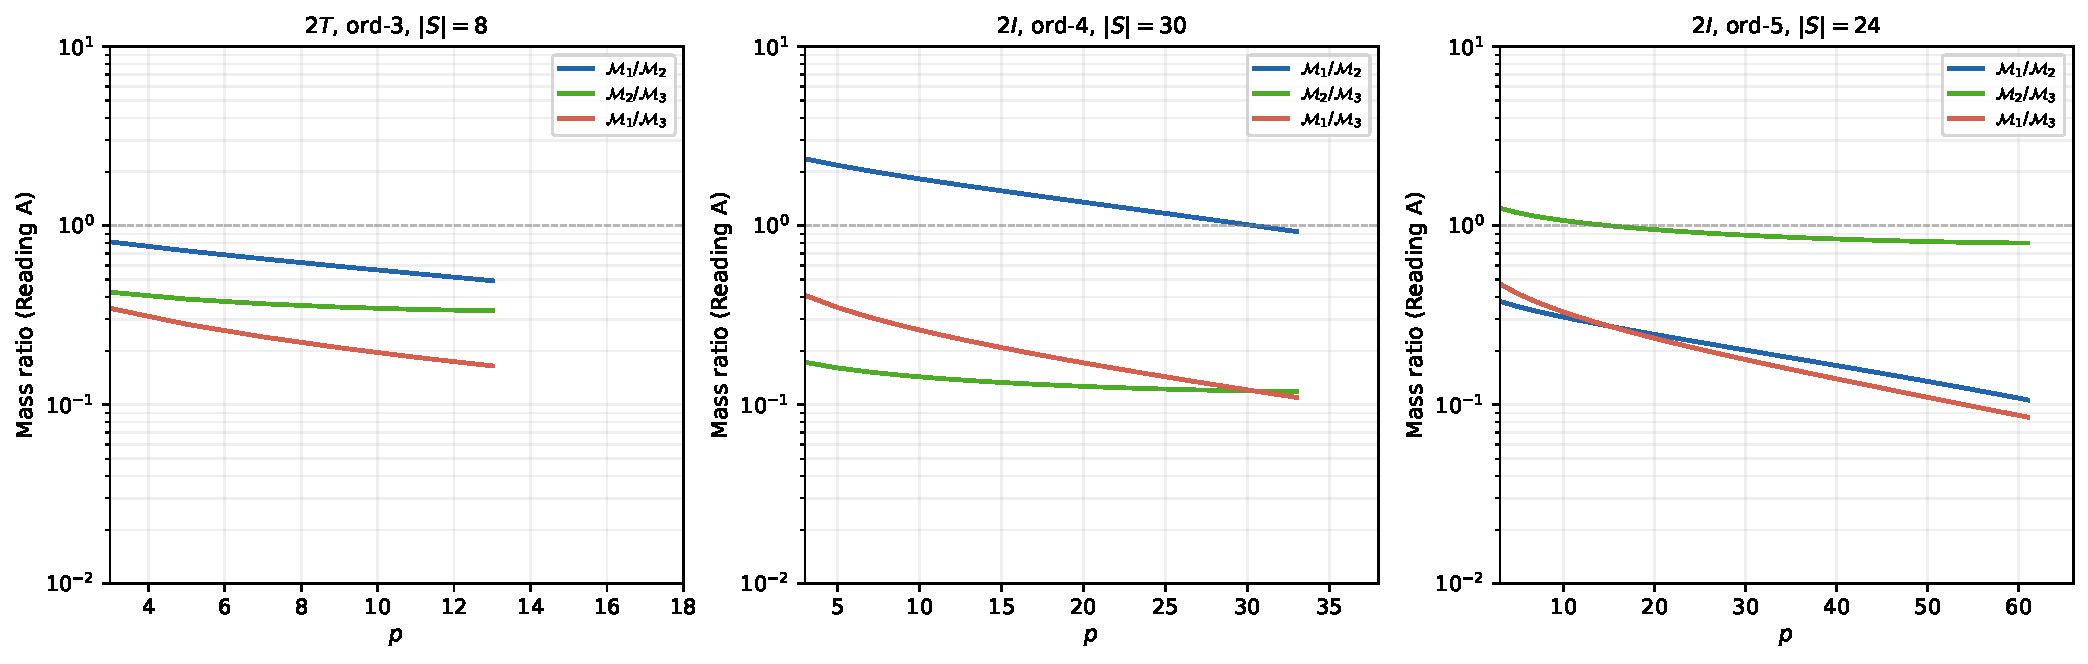
\includegraphics[width=0.90\textwidth]{../code/fig3_reading_A_ratios}
        \caption{Predicted $\log_{10}$ mass ratios under Reading~A
          ($\mathcal{M}_i \propto c_i/\dim\rho_i$) for $2I$ ord-4 (left)
          and $2I$ ord-5 (right), for all admissible primes $p$.
          Dashed horizontal lines show the observed Standard Model ratios
          for charged leptons, up-type quarks, and down-type quarks.
          The predicted ratios lie within $[-1, +1]$ on the log scale,
          whereas the observed ratios reach $-5$ for up-type quarks.}
        \label{fig:reading-A}
      \end{figure}

      The mass ordering depends on $c_i/\dim\rho_i$.
      In SpectralStratigraphy~\cite{Beau2026a4}, the admissibility envelope
      predicts $\mathcal{M}_1 > \mathcal{M}_2 > \mathcal{M}_3$ (lower $\lambda$ =
      heavier).
      The saturation mechanism predicts the opposite for $2I$ (ord-4): the level
      with largest $\lambda_3$ acquires the highest $c_3 \to 1$, giving
      $c_3/\dim\rho_3 \gg c_1/\dim\rho_1$.
      This inversion holds for all admissible $p$ and is a structural result, not a
      numerical accident.

    \subsection{Magnitude of the predicted hierarchy}
      \label{sec:amp:magnitude}

      All predicted ratios $\mathcal{M}_i/\mathcal{M}_j$ lie in $[0.10,\, 2.2]$.
      The observed ratios for Standard Model fermions range from $m_e/m_\mu \approx
  1/207$ to $m_u/m_t \sim 10^{-5}$.
      The best LPS--KM prediction ($\mathcal{M}_1/\mathcal{M}_3 \approx 0.10$ for
      $2I$ ord-5, $p=53$) falls short by approximately two orders of magnitude for
      leptons and four for up-type quarks.

    \subsection{Interpretation}
      \label{sec:amp:interpretation}

      \begin{quote}
        \emph{The LPS--Kesten--McKay saturation mechanism produces a well-defined
        three-level spectral stratification but fails to reproduce the observed
        inter-generation mass hierarchy, both in mass ordering and in magnitude.}
      \end{quote}

      The failure identifies two necessary extensions: a dynamical admissibility
      threshold and a supplementary amplification mechanism.
      Three open directions are described in Section~\ref{sec:disc:open}.
  \section{Discussion}
    \label{sec:discussion}

    \subsection{Status of the structural hypotheses}
      \label{sec:disc:hypotheses}

      \textbf{Hypothesis~\ref{hyp:closure}} identifies $c_{\mathrm{BI}}(n)$ with the
      isoperimetric capacity $h(G(n))$.
      It is the foundational physical postulate and currently lacks a derivation
      from the Cosmochrony axioms.

      \textbf{Hypothesis~\ref{hyp:saturation}} ($h^2 \asymp \lambda_2$) is a
      property of the graph family, consistent with but not implied by the Ramanujan
      property.
      It promotes $\Lambda_{\mathrm{proj}} \asymp h^2$ to the linear law
      $\Lambda_{\mathrm{proj}} \asymp \lambda_2$.

      \textbf{Hypothesis~\ref{hyp:saturation-rep}} ($M(\lambda_i) = k\,\dim\rho_i$,
      $k$ universal) is the only saturation condition internal to the framework that
      avoids free parameters.
      The constant $k$ cancels in all mass ratios.

      Of the three hypotheses, Hypothesis~\ref{hyp:closure} is the most in need of
      further justification.

    \subsection{Role of the parameter $p$}
      \label{sec:disc:p}

      The prime $p$ controls the Kesten--McKay support width via
      $\lambda_\pm = 1 \pm 2\sqrt{p}/(p+1)$.
      In the limit $p \to \infty$, the support collapses to $\{\lambda = 1\}$, so
      the spectral distribution becomes increasingly concentrated around the
      midpoint of the spectrum.
      Varying $p$ within the admissible range changes $c_i(p)$ quantitatively but
      not the qualitative conclusions: mass ratios remain of order one and the
      ordering inversion persists.
      The parameter $p$ should be regarded as a structural parameter of the
      cascade-graph model.
      A natural question is whether $p$ can be selected by the framework:
      the degree $d = p+1$ is related to the number of generators of
      $\mathrm{PSL}(2,\mathbb{F}_q)$ via the four-square decomposition of
      $p$~\cite{LPS1988}; a connection to the relational valence of the Cosmochrony
      cascade structure would constitute a selection principle.

    \subsection{Relation with SpectralStratigraphy}
      \label{sec:disc:stratigraphy}

      The two results of~\cite{Beau2026a4} used as inputs -- no-go for
      scalar calibration and three-level ADE structure -- are unaffected by the
      present analysis.

      The present work identifies two independent components of
      $n_{\mathrm{proj}}(\lambda)$: the admissibility support condition
      $\lambda \leq \Lambda_{\mathrm{proj}}$ and the saturation condition
      $N(\lambda; n) \geq k\,\dim\rho_\lambda$.
      The two mechanisms operate in different regimes.
      SpectralStratigraphy describes the regime in which $\Lambda_{\mathrm{proj}}(n)$
      evolves along the cascade; the present analysis shows that in the LPS model
      at fixed $p$ the threshold becomes asymptotically static, leaving saturation
      as the only active ordering mechanism.
      The admissibility ordering is recovered only when $\Lambda_{\mathrm{proj}}(n)$
      varies significantly, which requires a regime where $\lambda_2(n)$ is not
      asymptotically constant.

    \subsection{Interpretation of the numerical results}
      \label{sec:disc:numerical}

      The structural identity $c_2 = F_{\mathrm{KM}}(1) = 1/2$ holds for all $p$
      and all three-level ADE cases.
      It follows from the symmetry $\rho_{\mathrm{KM}}(\lambda) =
  \rho_{\mathrm{KM}}(2 - \lambda)$ of the Kesten--McKay density combined with
      the fact that the central ADE level always satisfies
      $\lambda_2^{\mathrm{norm}} = 1$.
      This coincidence is not accidental but follows from the combinatorial
      normalisation of the Laplacian together with the symmetry of the Kesten--McKay
      density.
      The identity $c_2 = 1/2$ is therefore a structural alignment between the
      spectral geometry of the projective substrate and the representation-theoretic
      structure of the ADE groups.

    \subsection{Open directions}
      \label{sec:disc:open}

      \medskip
      \noindent\textbf{(O1) Dynamical threshold via joint $p(n)$, $q$ variation.}

      \begin{figure}[h]
        \centering
        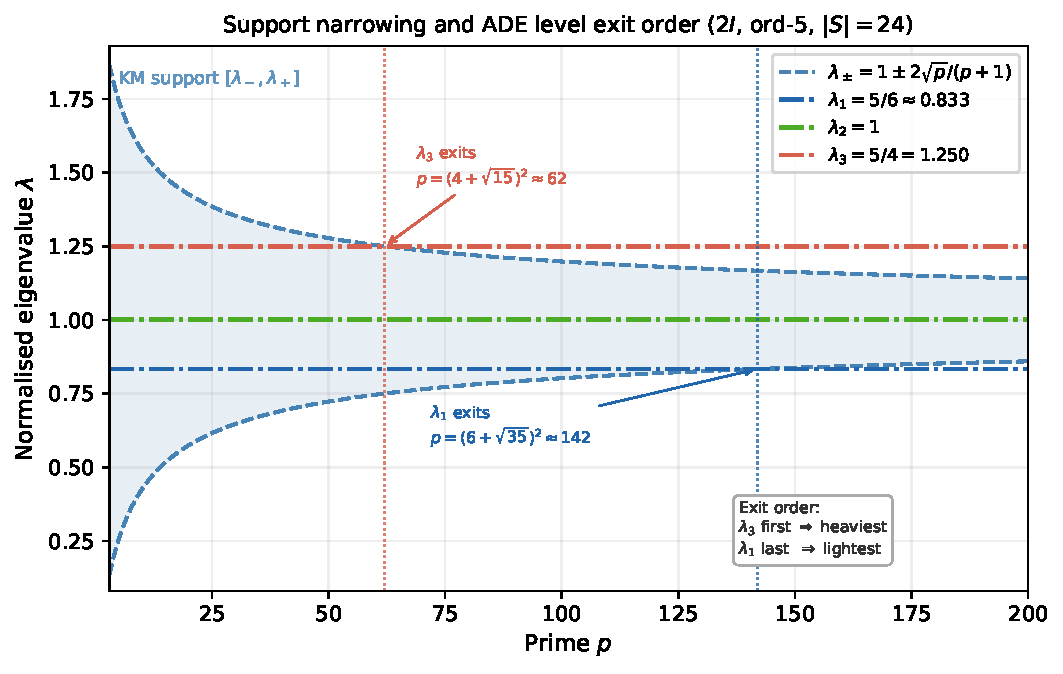
\includegraphics[width=0.72\textwidth]{../code/fig5_O1_support}
        \caption{Kesten--McKay support edges $\lambda_\pm(p) = 1 \pm 2\sqrt{p}/(p+1)$
          as functions of the prime $p$, with the three ADE eigenvalue levels of
          $2I$ (ord-5, $|S|=24$) shown as horizontal dash-dotted lines.
          As $p$ grows, the support \emph{narrows}: $\lambda_+ - \lambda_- =
          4\sqrt{p}/(p+1) \to 0$.
          The level $\lambda_3 = 5/4$ exits the support at $p = (4+\sqrt{15})^2 \approx 62$;
          $\lambda_2 = 1$ never exits (it is the midpoint of the symmetric support);
          $\lambda_1 = 5/6$ exits at $p = (6+\sqrt{35})^2 \approx 142$.}
        \label{fig:O1-support}
      \end{figure}

      If $p$ grows with $n$ -- for instance $p(n) \sim n^\beta$ for some $\beta > 0$,
      i.e.\ an effective increase of relational valence along the cascade -- then
      $\lambda_2^*(p) = 1 - 2\sqrt{p}/(p+1) \to 1$ and the Kesten--McKay support
      narrows with $n$.
      Such a joint scaling would correspond physically to an increase of the
      effective relational valence of the cascade structure along the cascade.
      This direction is the primary candidate for addressing both the ordering
      inversion and the amplitude problem simultaneously.

      A notable structural consequence of this mechanism concerns the ordering
      of stabilisation events.
      As $p(n)$ grows, the support $[\lambda_-, \lambda_+]$ narrows symmetrically
      around $\lambda = 1$.
      Since the ADE levels are fixed at $\lambda_1 < 1 < \lambda_3$, the level
      farthest from the centre exits the support first.
      For $2I$ (ord-5), the exit order is $\lambda_3$ (at $p \approx 62$), then
      $\lambda_1$ (at $p \approx 142$), while $\lambda_2 = 1$ never exits.
      A level that exits the support is no longer admissible and stabilises at
      the corresponding cascade rank; earlier exit therefore corresponds to higher
      stabilisation mass.
      The resulting mass ordering is $\mathcal{M}_3 > \mathcal{M}_1 >
  \mathcal{M}_2$, which for the physically relevant assignment
      $\lambda_3 \leftrightarrow$ first generation restores the hierarchy
      expected from the admissibility envelope of~\cite{Beau2026a4},
      without any additional dynamical hypothesis.
      This ordering result is a direct structural implication of the support
      narrowing and is independent of the precise growth law $p(n)$.

      \medskip
      \noindent\textbf{(O2) Hierarchical cascade.}
      If the saturation process operates recursively across $L$ nested levels, the
      per-level ratio $r$ yields $r^L$.
      With $r \approx 0.1$ and $L = 3$, one obtains $r^3 \approx 10^{-3}$,
      approaching the lepton mass ratio $m_e/m_\tau \approx 3 \times 10^{-4}$.

      \medskip
      \noindent\textbf{(O3) Sub-linear energy-rank relation.}
      Replacing $E_n = E_{\mathrm{P}}/n$ by $E_n = E_{\mathrm{P}}/n^\alpha$ with
      $\alpha < 1$ modifies the ratios to
      $(c_i\,\dim\rho_j)^\alpha / (c_j\,\dim\rho_i)^\alpha$.
      This reduces the amplitude problem but preserves the ordering inversion, so it
      does not constitute a complete solution.

      \medskip
      \noindent\textbf{Cosmological expansion and the two growth regimes.}
      The total projectable mode count $N_{\mathrm{proj}}(n)$ grows as a function of
      the cascade rank $n$.
      In the present LPS model at fixed $p$, this growth is linear
      (Proposition~\ref{prop:Nproj-linear}).
      In the O-series Heisenberg BFS model, two distinct growth regimes are
      structurally present:
      \begin{itemize}
        \item a \emph{polynomial regime}, in which individual BFS shells grow as
        $|S_n| \sim n^3$ (Bass--Guivarc'h, homogeneous dimension $D_{\mathrm{hom}} = 4$),
        governing the early cascade;
        \item an \emph{exponential regime}, carried by the branching of admissible
        trajectories, governing the late cascade once the spectral position is
        sufficiently displaced from the origin.
      \end{itemize}
      The precise carrier of the exponential regime on the Heisenberg substrate is
      determined in the trajectory-branching note~\cite{Beau2026tb}.
      Any identification of $N_{\mathrm{proj}}(n)$ with an endpoint-based count
      (ball volumes, fibre registers, or any function of the final Heisenberg
      element) inherits the polynomial Bass--Guivarc'h growth and cannot sustain
      the exponential regime; the regime survives at the level of
      \emph{projectively distinguishable histories}: trajectories separated by
      their projected residual profiles rather than by their endpoints.
      For the canonical channel compatible with the exact Weil-block pipeline, the
      distinguishable-history count follows the Pell recurrence
      $N(n) = 2N(n-1) + N(n-2)$, with asymptotic rate
      $h_b = \log(1+\sqrt{2})$~\cite{Beau2026tb}.
      These two regimes provide a structural two-phase model for cosmic expansion:
      decelerated growth in the polynomial regime --- where the early profiles are
      still projectively degenerate --- transitioning to accelerated growth in the
      exponential (history-branching) regime.
      The transition between regimes occurs naturally as the accumulated projective
      divergence $I(n)$ crosses the threshold at which the branching factor dominates
      the individual shell growth.
      Under this identification, the cosmological ``dark energy'' is not a vacuum
      energy field but the structural pressure of an expanding space of admissible
      reprojections --- a direct consequence of the recursive admissibility law
      $O_{n-1} \to O_n \to \mathcal{A}(O_n) \to O_{n+1}$ established
      in~\cite{Beau2026m}.

      This picture is structurally compatible with recent observational evidence from
      DESI~\cite{DESI2025} suggesting that dark energy is not a cosmological constant
      but weakens over cosmic time ($w_0 > -1$, $w_a < 0$ in the $w_0 w_a$CDM
      parametrisation).
      In the two-regime model, the effective equation-of-state parameter $w(n)$
      evolves as the branching of distinguishable histories is progressively
      compressed by the accumulated projective history; the candidate carrier of
      this evolution is the full-history compression profile identified
      in~\cite{Beau2026tb}, whose cosmological use remains conditional on a
      canonical identification of the full-history projective observable.
      The remaining step --- the dictionary between cascade rank and cosmic time,
      and between the distinguishable-history count and the expanding observable
      --- is deferred to the Cosmology companion paper.

  \section{Conclusion}
    \label{sec:conclusion}

    This paper analysed the spectral mechanism governing the projective resolution
    along the projective cascade within an LPS Ramanujan graph model, and established
    that this mechanism, at fixed prime~$p$, is insufficient to produce the observed
    mass hierarchy.
    The identification of this structural obstacle --- the asymptotic constancy of
    $\Lambda_{\mathrm{proj}}$ --- was historically the starting point of the O-series,
    which adopted the Heisenberg BFS cascade on
    $\mathrm{Heis}_3(\mathbb{Z}/q\mathbb{Z})$ as its concrete cascade model precisely
    because it provides a dynamical $\sigma_{\mathrm{pair}}(n)$ that decays rather
    than saturates.
    The derivation of the mass hierarchy rests on the O-series transfer chain
    $c_{\mathrm{BI}} \to \delta_{\mathrm{pair}} \to \beta^*$~\cite{Beau2026a28,Beau2026a29};
    the present results identify the structural obstacle and the open direction that the
    O-series addresses.
    The companion paper~\cite{Beau2026a4} established that the
    representation-theoretic structure of ADE binary Cayley graphs fixes the
    number and order of stratigraphic levels, while the dynamical growth of
    $\Lambda_{\mathrm{proj}}(n)$ controls their separation.
    The present paper addresses this second question within the LPS model.

    The main positive results are: the isoperimetric law
    $\Lambda_{\mathrm{proj}}(n) \asymp h(G(n))^2$
    (Proposition~\ref{prop:Lambda-h}); the Cheeger enclosure
    $\lambda_2^2 \lesssim \Lambda_{\mathrm{proj}} \lesssim \lambda_2$
    (Corollary~\ref{cor:cheeger-enclosure}); the linear law
    $\Lambda_{\mathrm{proj}} \asymp \lambda_2$ under spectral-isoperimetric
    saturation (Corollary~\ref{cor:linear-law}); the linear growth
    $N(\lambda; n) \sim F_{\mathrm{KM}}(\lambda) \cdot n$
    (Proposition~\ref{prop:Nproj-linear}); and the factorised mass ratio formula
    \[
      \frac{\mathcal{M}_i}{\mathcal{M}_j}
      \;=\;
      \frac{F_{\mathrm{KM}}(\lambda_i)}{F_{\mathrm{KM}}(\lambda_j)}
      \cdot
      \frac{\dim\rho_{\lambda_j}}{\dim\rho_{\lambda_i}},
    \]
    in which the structural identity $F_{\mathrm{KM}}(1) = 1/2$ holds universally.

    Two limitations are established: the saturation mechanism inverts the mass
    ordering expected from the admissibility envelope, and the predicted mass
    ratios lie in $[0.10,\, 2.2]$, far below the observed $10^{-3}$--$10^{-5}$
    range.
    Both limitations are traced to the asymptotic constancy of
    $\Lambda_{\mathrm{proj}}$ in the LPS model at fixed $p$.

    The primary open direction is direction~(O1): allowing $p(n) \to \infty$ with
    $n$, so that the Kesten--McKay support narrows progressively, the ADE levels
    leave the support in a rank-dependent order, and the admissibility and
    saturation conditions are coupled.
    This regime, in which the effective relational valence of the cascade structure
    increases along the cascade, is the natural candidate for recovering both the
    correct mass ordering and the observed amplification, and will be the subject
    of the next paper in the admissibility sub-programme.

    \clearpage
    \bibliographystyle{plain}
    \bibliography{cosmochrony-bibliography,external-refs}

\end{document}
